\begin{question}
\noindent A biologist is examining a specimen under a microscope. The outline of a bacterium, shape $S$, is plotted on the grid below, which represents the squares etched onto the slide.

The biologist shifts the slide so that the specimen's image moves according to the column vector $\begin{pmatrix} 3 \\ -2 \end{pmatrix}$.

\begin{center}
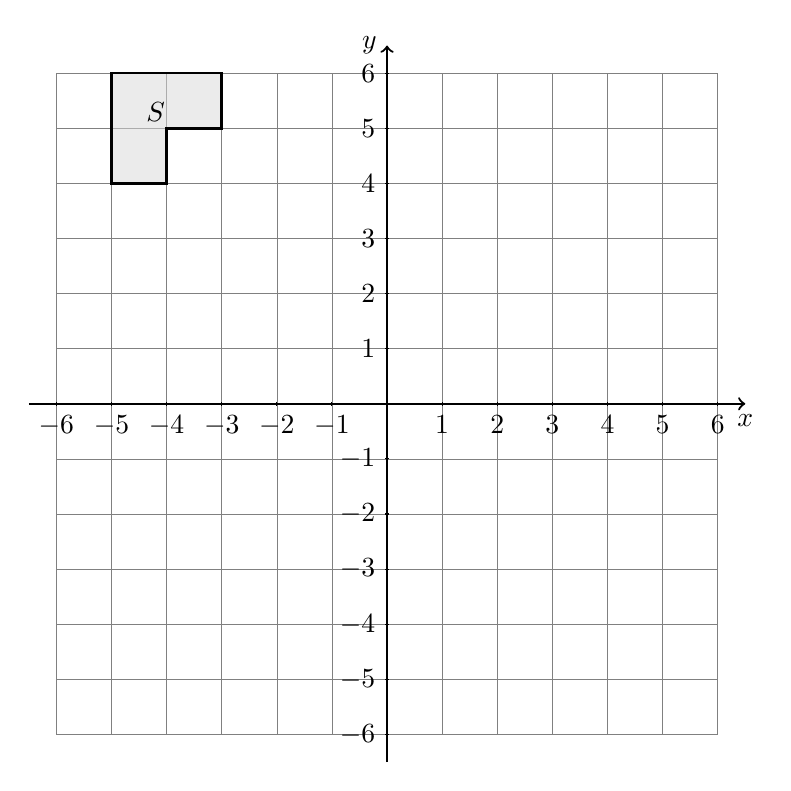
\begin{tikzpicture}[scale=0.7]
    % Define colours
    \definecolor{borderColour}{HTML}{000000}
    \definecolor{fillColour}{HTML}{D8D8D8}

    % Define axis scale
    \def\axisLimit{6}

    % Draw the grid
    \draw[step=1cm,gray,very thin] (-\axisLimit,-\axisLimit) grid (\axisLimit,\axisLimit);
    \draw[thick,->] (-\axisLimit-0.5,0) -- (\axisLimit+0.5,0) node[anchor=north] {$x$};
    \draw[thick,->] (0,-\axisLimit-0.5) -- (0,\axisLimit+0.5) node[anchor=east] {$y$};

    % Label x-axis
    \foreach \x in {-6,-5,...,-1,1,2,...,6}
        \draw (\x cm,1pt) -- (\x cm,-1pt) node[anchor=north] {$\x$};
    % Label y-axis
    \foreach \y in {-6,-5,...,-1,1,2,...,6}
        \draw (1pt,\y cm) -- (-1pt,\y cm) node[anchor=east] {$\y$};

    % Define the vertices of shape S
    \coordinate (A) at (-5,4);
    \coordinate (B) at (-5,6);
    \coordinate (C) at (-3,6);
    \coordinate (D) at (-3,5);
    \coordinate (E) at (-4,5);
    \coordinate (F) at (-4,4);

    % Draw shape S
    \filldraw[fill=fillColour, draw=borderColour, line width=1pt, fill opacity=0.5] (A) -- (B) -- (C) -- (D) -- (E) -- (F) -- cycle;

    % Label shape S
    \node[left] at (A) {};
    \node at (-4.2,5.3) {$S$};

\end{tikzpicture}
\end{center}

\noindent On the grid, draw the image of shape $S$ after a translation by the vector $\begin{pmatrix} 3 \\ -2 \end{pmatrix}$.

Label the image $S'$.

\vspace{4cm}
\begin{flushright}
    \answermarks{3}
\end{flushright}
\end{question}
